\subsection{Coisas dentro da Wikipédia}

Seguindo esta trilha então narramos esforços da comunidade wikipedista de melhorar a recepção de novatos, como o Teahouse (MORGAN e HALFAKER, 2018), espaço na Wikipédia anglófona que funciona como um fórum com tutores e usuários novatos, e o Snuggle (HALFAKER et al., 2014), que segundo a Wikipédia (WiKIPEDIA-PT, “Wikipédia:Snuggle”, 07/07/2014) ”é um sistema web para observação e apoio a novatos [...] desenvolvido para permitir que tutores observem as atividades de usuários recém registrados separando novatos desejáveis (boa fé e produtivo (sic)) de indesejáveis (má fé e vândalos)”, a iniciativa "Wikipedia Adventure" (NARAYAN et al., 2017) e o robô ClueBot NG.


\begin{figure}[H]
    \centering
    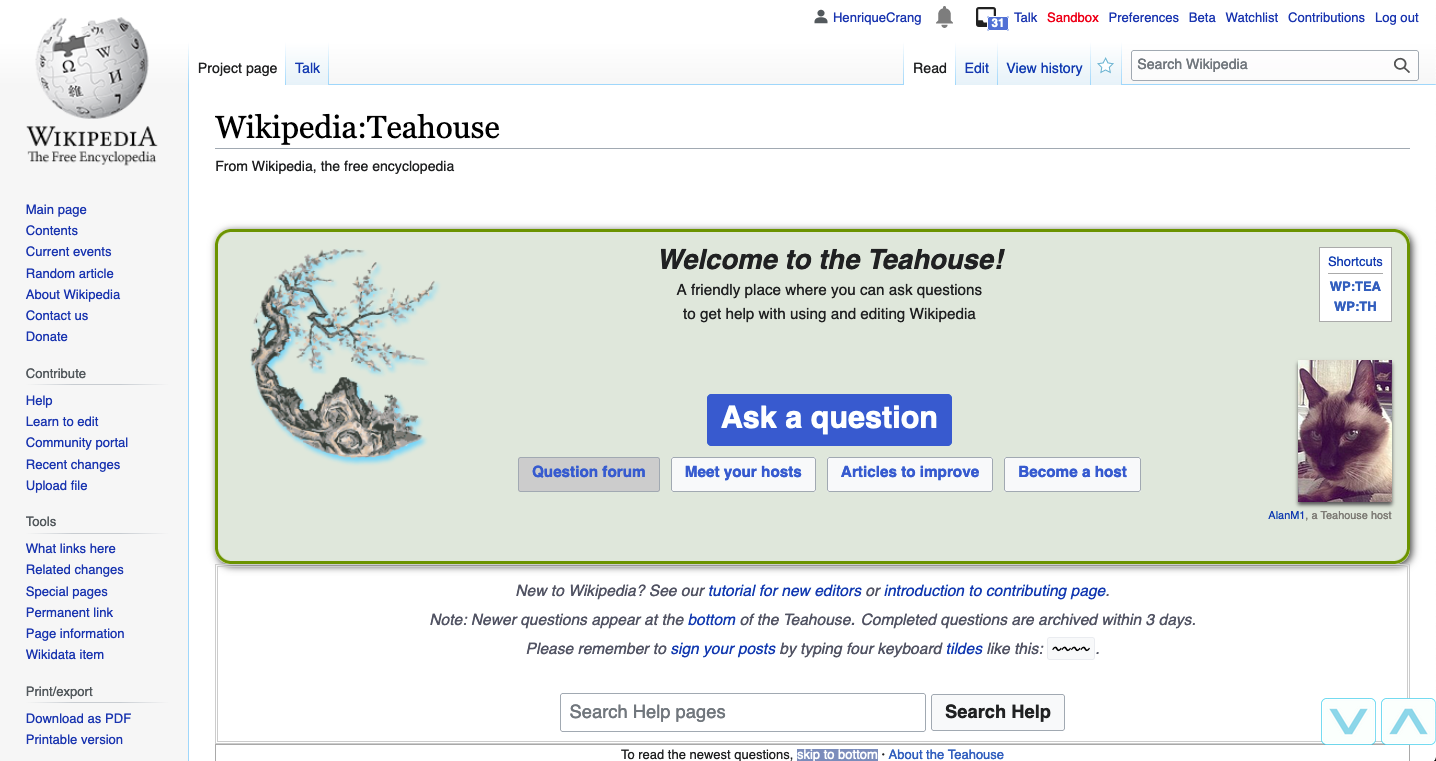
\includegraphics[width=1\textwidth]{Images/en_wikipedia_teahouse.png}
    \caption{Página da Teahouse na Wikipédia em inglês.}
    \label{fig:teahouse}
\end{figure}


# Dificuldade de usuários novos: vários casos de sucesso da TeaHouse na enwiki, mas na ptwiki o "Café dos novatos", que foi renomeado para https://pt.wikipedia.org/wiki/Wikip%C3%A9dia:Tire_suas_d%C3%BAvidas é muito pouco usado e nada linkado.
# Posso comparar número de uso do café na en e na ptwiki


# Falar sobre Wikipedia Adventure (NARAYAN et al., 2017)
# usar (TARABORELLI e CIAMPAGLIA, 2015)

\begin{figure}[H]
    \centering
    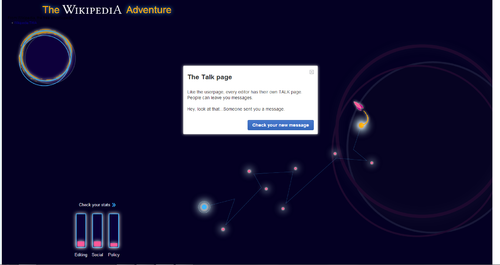
\includegraphics[width=1\textwidth]{Images/en_wikipedia_adventure.png}
    \caption{Página do Wikipédia Adventure na Wikipédia em Inglês.}
    \label{fig:wp_adventure}
\end{figure}




# falar do Snuggle (tenho algum texto sobre isso em algum lugar, talvez na qualificação, quando falo do caminho dos MAM).

\begin{figure}[H]
    \centering
    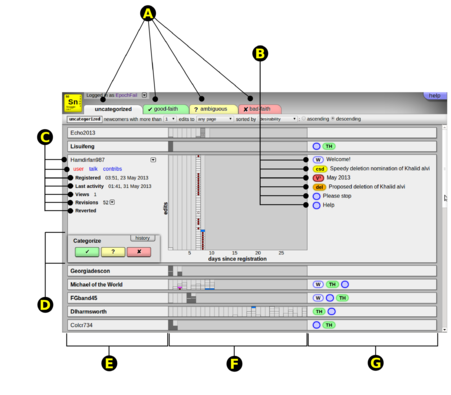
\includegraphics[width=1\textwidth]{Images/snuggle.png}
    \caption{Página do Snuggle.}
    \label{fig:snuggle}
\end{figure}


